\documentclass[10pt]{beamer}
\usetheme{Warsaw}
\title{Implementation of Cuckoo Search Algorithm}
\author{Guided by : Anuraj Mohan}
\institute[UMBC]{Mini Project Presentation \\
  Department of Computer Science and Engineering \\
  NSS College of Engineering \\
  Palakkad \\

}
\date{April 02, 2012}
\begin{document}

%----Title----%

\begin{frame}[plain]
  \titlepage
\end{frame}

\begin{frame}
	\frametitle{Group Members}
	\begin{itemize}
	\item Anand Krishnan R - 08
	\item Anoop Gopan - 10
	\item Ashik Salman P - 16
	\item Lal Krishna Raj - 32
	\end{itemize}
\end{frame}	
%----Slides----%
%-1-%
\begin{frame}
  \begin{columns}
    \begin{column}{0.1\textwidth}
      \textbf{What!?}
    \end{column}
  \end{columns}
\end{frame}

%-2-%
\begin{frame}
  \frametitle{Context}
  \textbf{Let's discuss something NEW..!!}
  \medskip
  \begin{itemize}
    \item Algorithms.
    \pause
    \item Swarm Intelligence.
    \pause
    \item Nature Inspired Algorithms.
    \pause
    \item Intractable problems.
    \pause
    \item Optimization Algorithms.
    \begin{itemize}
    	\item PSO.
    	\item ACO.
    	\item DE.
    	\item GA.
    	\item ABC.
    \end{itemize}
  \end{itemize}
\end{frame}

%-2-%
\begin{frame}
  \frametitle{Abstract}
  \textbf{Cuckoo Search Algorithm}
  \medskip
  \pause
  \begin{itemize}
    \item New Metaheuristics optimisation algorithm.
    \pause
    \item Implementation in Python.
    \pause
    \item Comparative study with existing MATLAB implementation.
    \pause
    \item Future Scope.
  \end{itemize}
\end{frame}

\begin{frame}
  \frametitle{System Specification}
  \textbf{Software Requirements}
  \begin{itemize}
  	\item Front end : Tkinter module in Python.
    \item Back end   : Python 2.7.1+
    \item Platform    : Linux.
  \end{itemize}
  \textbf{Hardware Requirements}
  \begin{itemize}
  	\item Processor : Intel Pentium 4 or above.
  	\item RAM	       : 2 GB or above
  	\item Hard Disk : 1 GB free space or more
  \end{itemize}	
\end{frame}


%-3-%
\begin{frame}
  \frametitle{Introduction}
  \textbf{Cuckoo Search}
  \medskip
  \begin{itemize}
  	\pause
  	\item Developed by Yang & Deb in 2009.
  	\pause
  	\item Finds Optimal solutions.
  	\pause
  	\item Two efficient implementations have been introduced.
  	\pause
    \item Yang and Deb implemented CS in MATLAB.
    \pause
    \item Nebojsa Bacanin developed an object oriented version in JAVA.
  \end{itemize}
\end{frame}

%-4-%
\begin{frame}
  \frametitle{CS Algorithm}
  \textbf{Why it is "Cuckoo" Search..?}
  \begin{itemize}
  	\pause
  	\item Breeding behaviour of Cuckoo Species.
  	\pause
    \item Random walk.
    \pause
    \item Mimics host's egg.
    \pause
    \item Survives unless NOT found by HOST.
    \pause
    \item Mimics call of host chicks.
  \end{itemize}
\end{frame}

%-5-%
\begin{frame}
  \frametitle{Implementation}
  \textbf{Four Phases.}
	 \begin{itemize}
	 	\pause
    	\item Understanding Algorithm Concepts.
    	\pause
	    \item Mapping to Python. 
	    \pause
        \item GUI Development.
        \pause
        \item Comparison study.
     \end{itemize}
\end{frame}

\begin{frame}
  \frametitle{Implementation}
  \textbf{Python.}
  \begin{itemize}
  	\item General purpoes High Level Language.
    \item Interpreted Language.
    \item Supports Multi paradigm.
    \item Rich in library function.
    \item Pylab and Mayavi to Plot 
   \end{itemize}
   \textbf{TKinter}
   \begin{itemize}
   	\item Ease of use and design.
  \end{itemize}
\end{frame}


%-6-%

\begin{frame}
	\frametitle{Algorithm}
	\textbf{Cuckoo Search}
	\begin{center}
	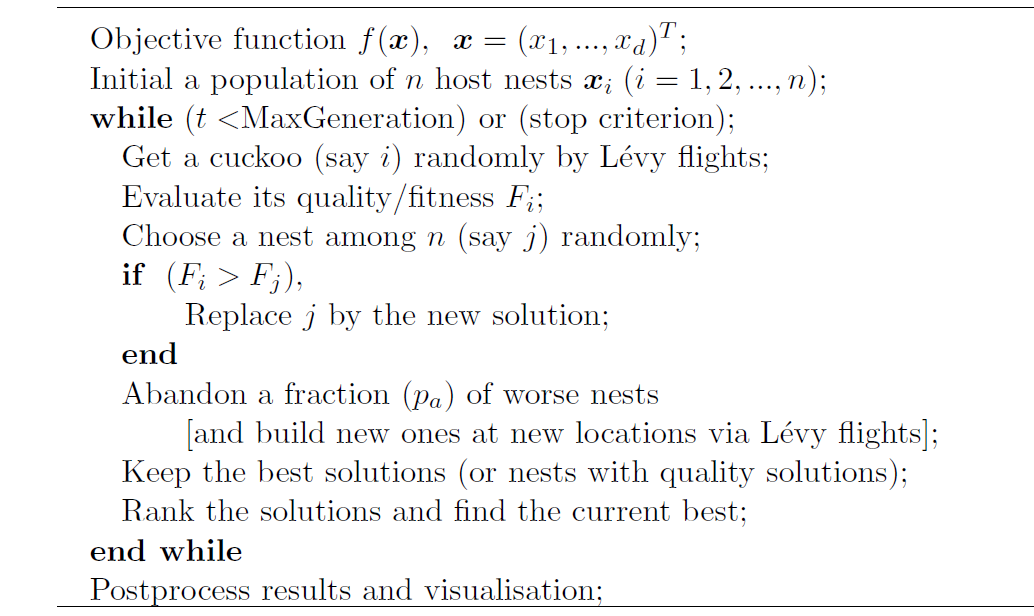
\includegraphics[width=1.0\textwidth]{ab.png}
	\end{center}
\end{frame}

\begin{frame}
  \frametitle{Implementation}
  \textbf{Understanding Algorithm Concepts.}
  \begin{itemize}
    \item Creating random candidate solutions.
    \item Checking for the fitness of solutions.
    \item Getting a minimum value.
    \item If min value meets the tolerance condition stop iteration.
    \item Else create a set by Levy flight \\ and checks iteratively for a better solution.
  \end{itemize}
\end{frame}



	
\begin{frame}
	\frametitle{Data Flow Diagram}
	\textbf{How it works..?}
	\begin{center}
	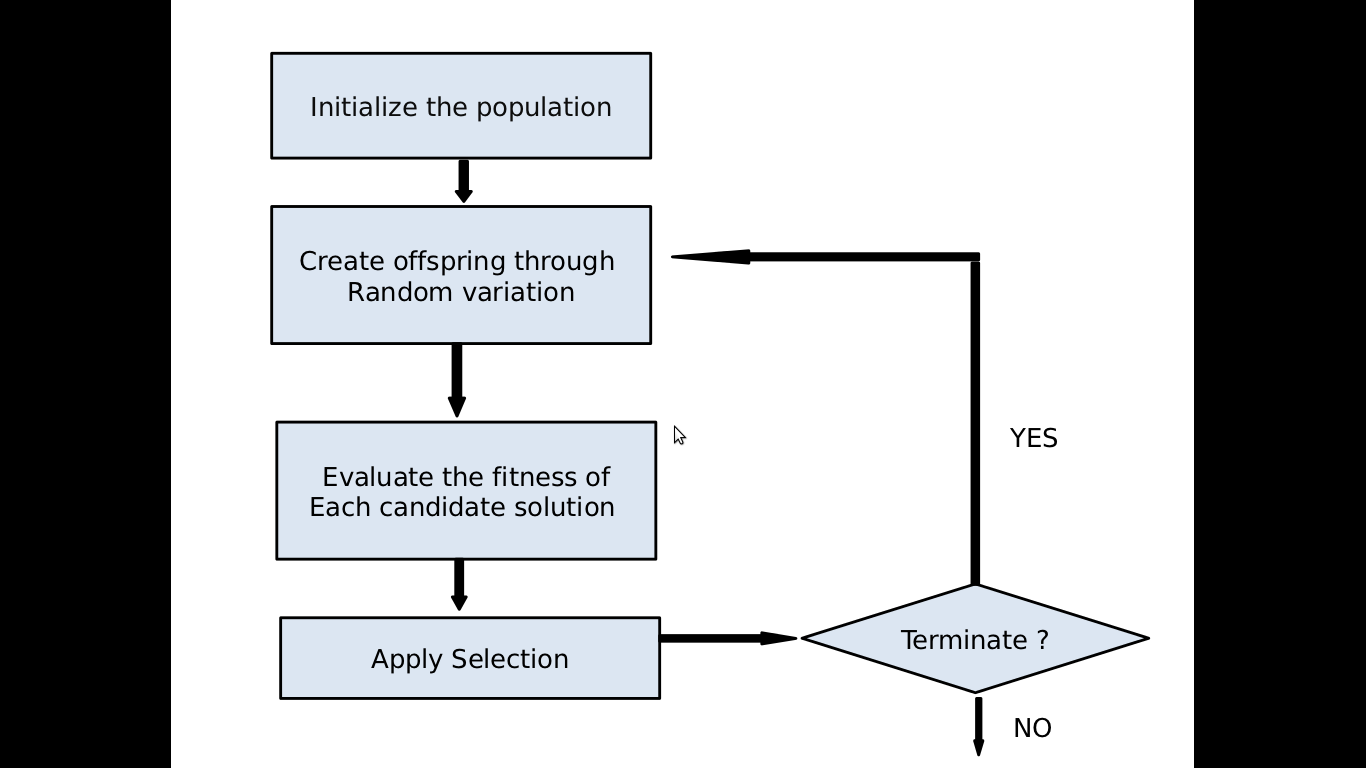
\includegraphics[width=1.0\textwidth]{aa.png}
	\end{center}
\end{frame}

\begin{frame}
	\frametitle{Algorithm}
	\textbf{What actually happens}
	\begin{center}
	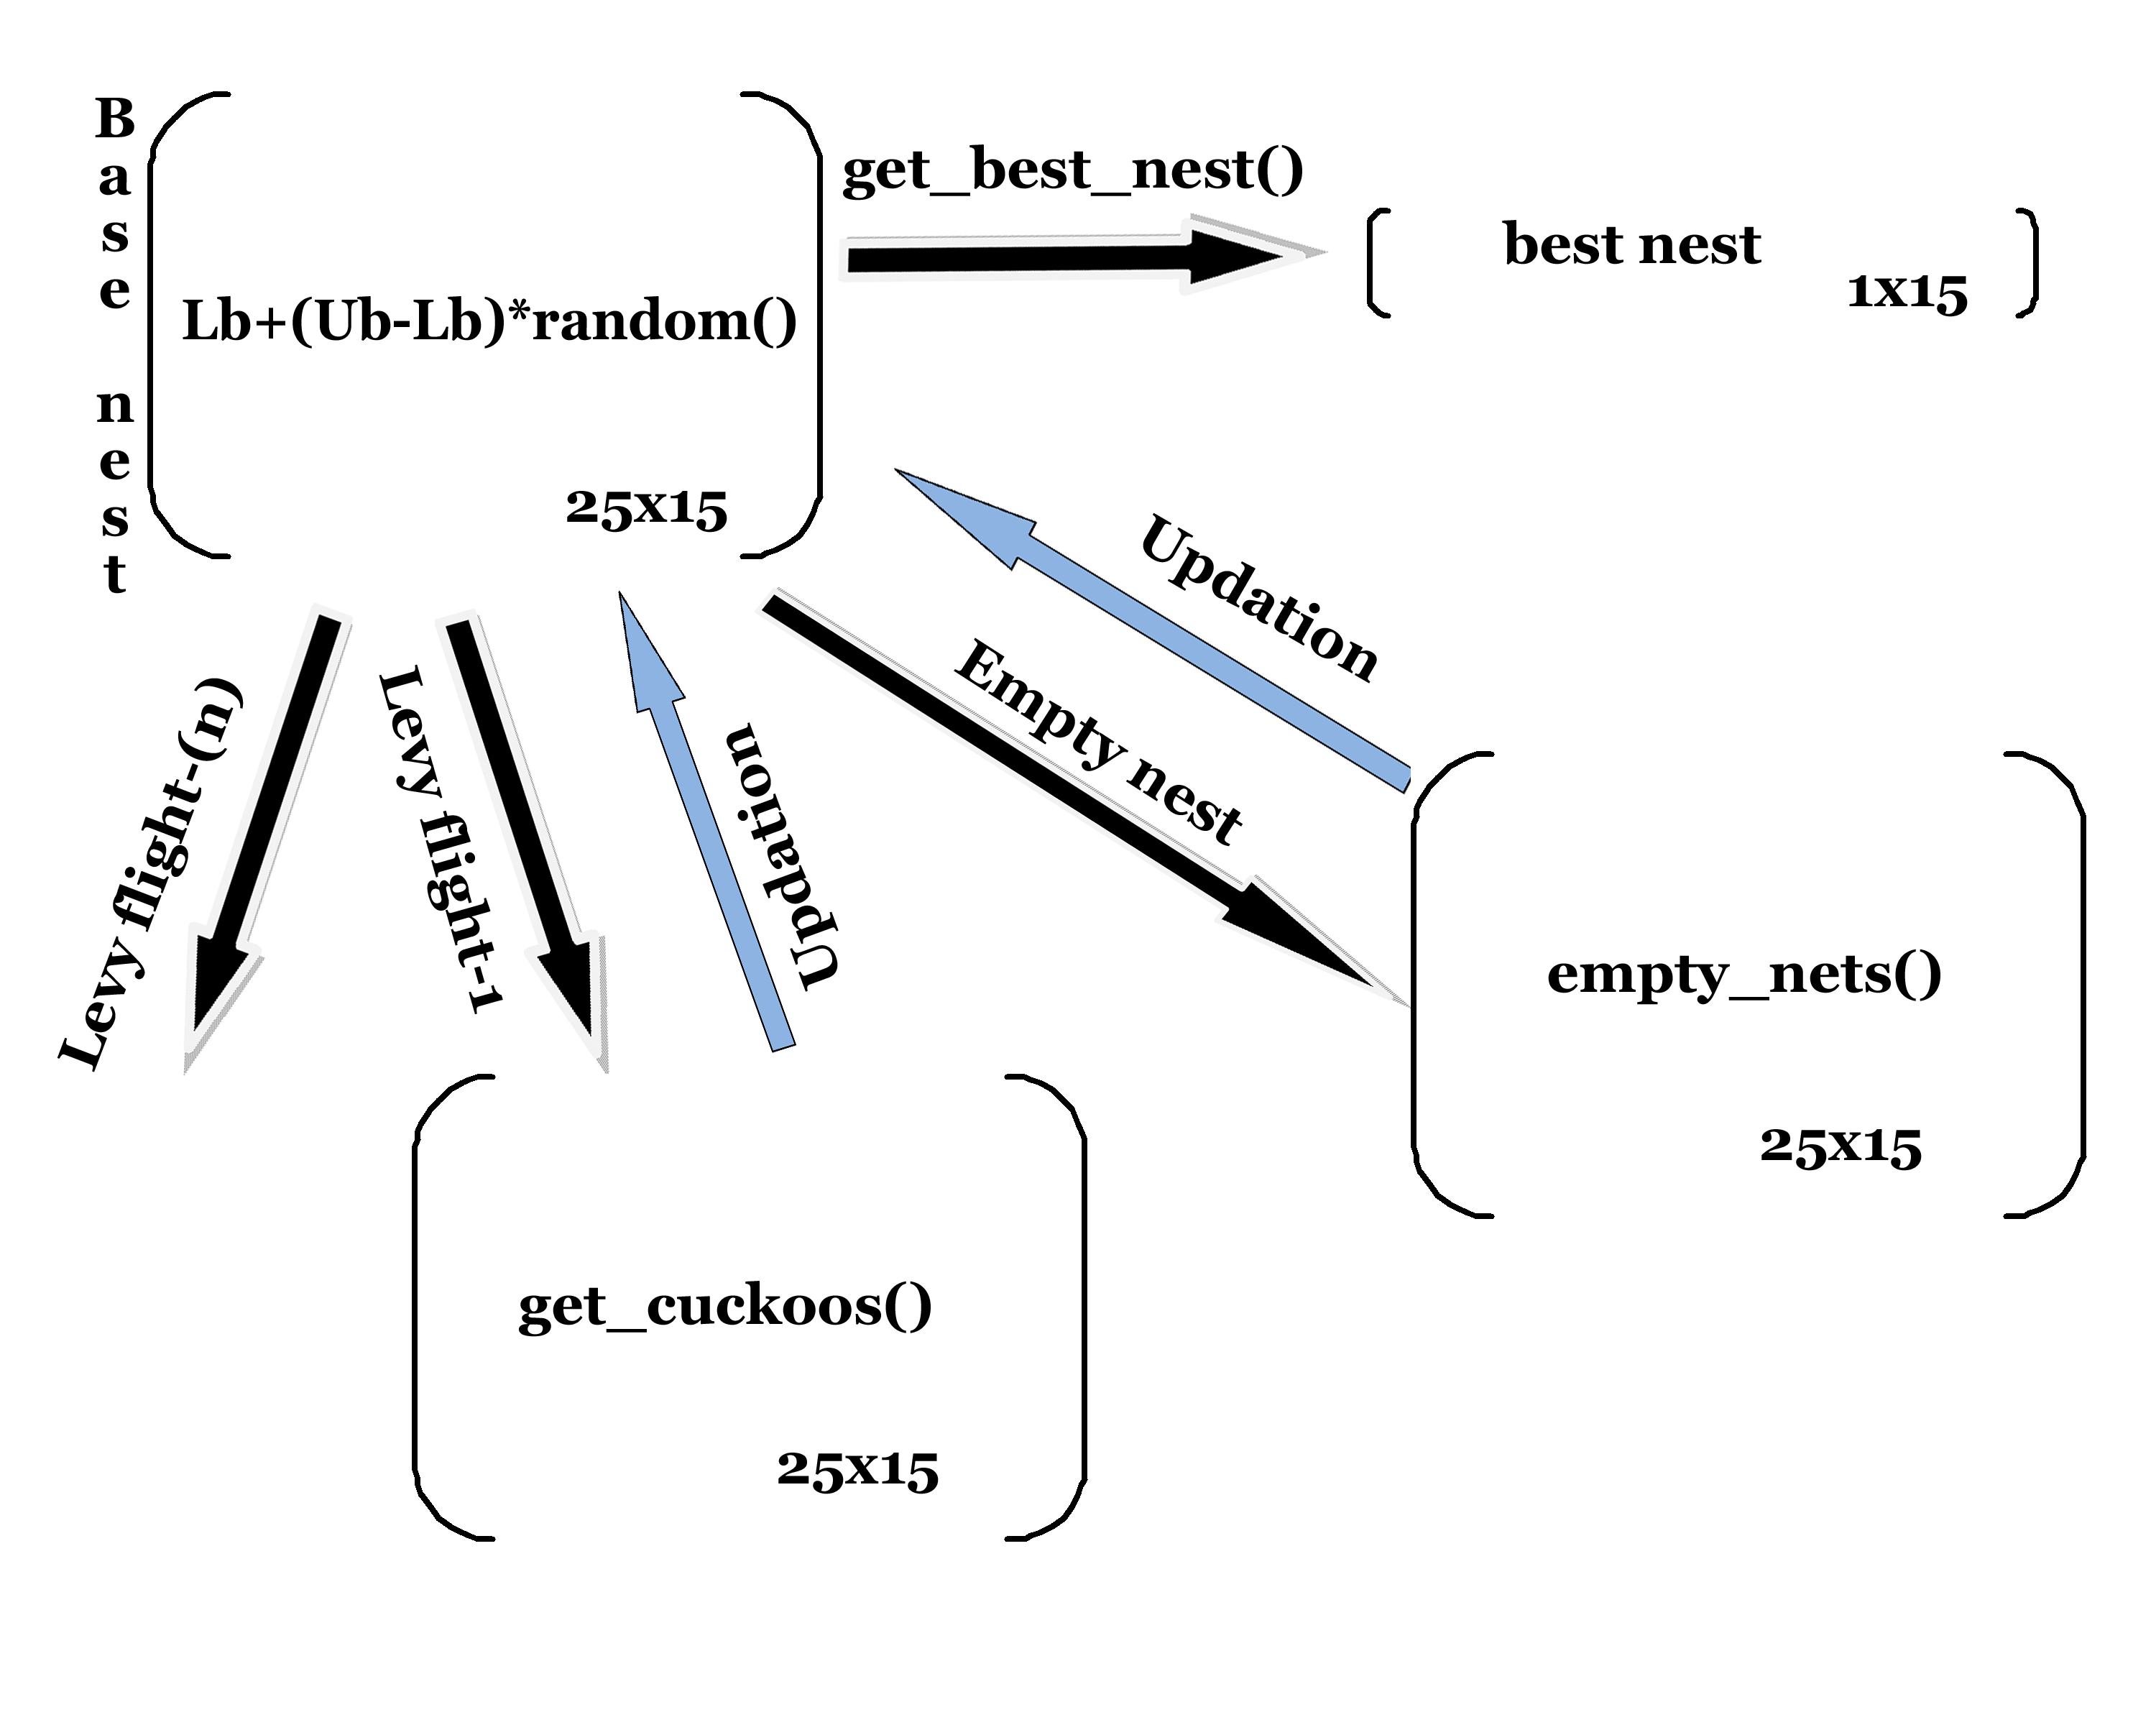
\includegraphics[width=0.90\textwidth]{ae.png}
	\end{center}
\end{frame}
	
\begin{frame}
  \frametitle{Implementation}
  \textbf{Mapping to Python.}
  \begin{itemize}
    \item Representing Nests as arrays and Matrices.
    	\begin{itemize}
    	\item Python Numpy Module - ease of math operations.
    	\end{itemize}
    \item Creating initial random candidate solution set.
    	\begin{itemize}
    	\item Python Random module - generates random variables.
    	\end{itemize}
    \item User defined functions.
    	\begin{itemize}
    	\item get-best-nest, get-cuckoos, empty-nest etc.
    	\end{itemize}
    \item Loops
    	\begin{itemize}
    	\item Checks iteratively to meet tolerance condition.
    	\end{itemize}
    \item Output.
    	\begin{itemize}
    	\item Prints fmin, best-nest, execution time, iterations.
    	\end{itemize}
  \end{itemize}
\end{frame}




%-9-%
\begin{frame}
  \frametitle{Conclusion}
  In this project we have implemented Cuckoo Search Algorithm in Python and tested using Sphere function, a standard benchmark.\\
  \medskip
  \textbf{Result}
  \begin{itemize}
  	\item Testing using Sphere function resulted in obtaining optimization of function.
  	\item It is found that Cuckoo Search Algorithm can outperform the existing Metaheuristics algorithms.
  	\item The optimal solution obtained by CS are far better than the best solutions obtained by an efficient PSO.
  	\begin{itemize}
  	\item Courtesy : Engineering optimisation by Cuckoo Search,\\ IEEE arXiv:1005.2908v3 [math.OC] 23 Dec 2010.
  	\end{itemize} 
  \end{itemize}
  \textbf{Performance.}
  \begin{itemize}
    \item Promising results obtained with minimum number of iterations.	
  \end{itemize}  
\end{frame}

%-10-%
\begin{frame}
  \frametitle{Application.}
  \textbf{Engineering Optimization Problems.}
  \begin{itemize}
  	\item Spring Design.
  	\begin{center}
  	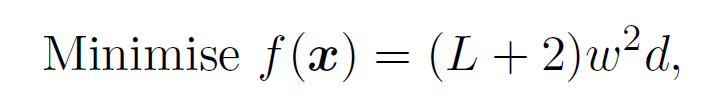
\includegraphics[width=0.60\textwidth]{ac.png}
  	\end{center}
  	\item Welded Beam.
  	\begin{center}
  	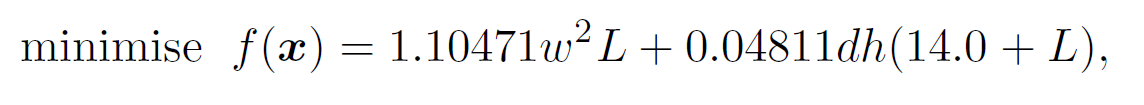
\includegraphics[width=0.80\textwidth]{ad.png}
  	\end{center}
  \end{itemize}
  \textbf{Nurse Scheduling Problems}\\
\end{frame}

\begin{frame}
	\frametitle{Future Scope}
	\begin{itemize}
	\item Data Fusion In Wireless Sensor Networks.
	\item Modified CS Algorithm is a powerful gradient free optimisation algorithm.
	\item Can be integrated with many existing optimisation algorithms to get better performance.
	\end{itemize}
\end{frame}


%-11-%
\begin{frame}
  \frametitle{Contribution by members.}
  \textbf{Ashik Salman P\\ Lal Krishna Raj}
  \begin{itemize}
  	\item Understanding Algorithm Concepts and MATLAB implementation.
  \end{itemize}
  \textbf{Anand Krishnan R}
  \begin{itemize}
  	\item Coding in Python.
  \end{itemize}
  \textbf{Anoop Gopan}
  \begin{itemize}
  	\item Comparison Study.
  \end{itemize}
\end{frame}

%-12-%
\begin{frame}
  \frametitle{Reference}
  \begin{itemize}
  	\item Engineering Optimisation by Cuckoo Search - \\
  	Paper presented by Xin-She Yang and Suash Deb.
  	\begin{itemize}
  	\item IEEE reference : arXiv: 1005.2908v3 [math.OC] 23 Dec 2010.
  	\end{itemize}
  	\item An Object-oriented software implementation of a novel cuckoo search algorithm - paper presented by Nebojsa Bacanin.
  	\begin{itemize}
  	\item Proceedings of the European Computing Conference, Ministry of Science, Republic of Serbia, Project No. 44006
  	\end{itemize}
	\end{itemize}	  
\end{frame}

\begin{frame}
	\frametitle{Screen Shots}
	\textbf{Code Execution}
	\begin{center}
	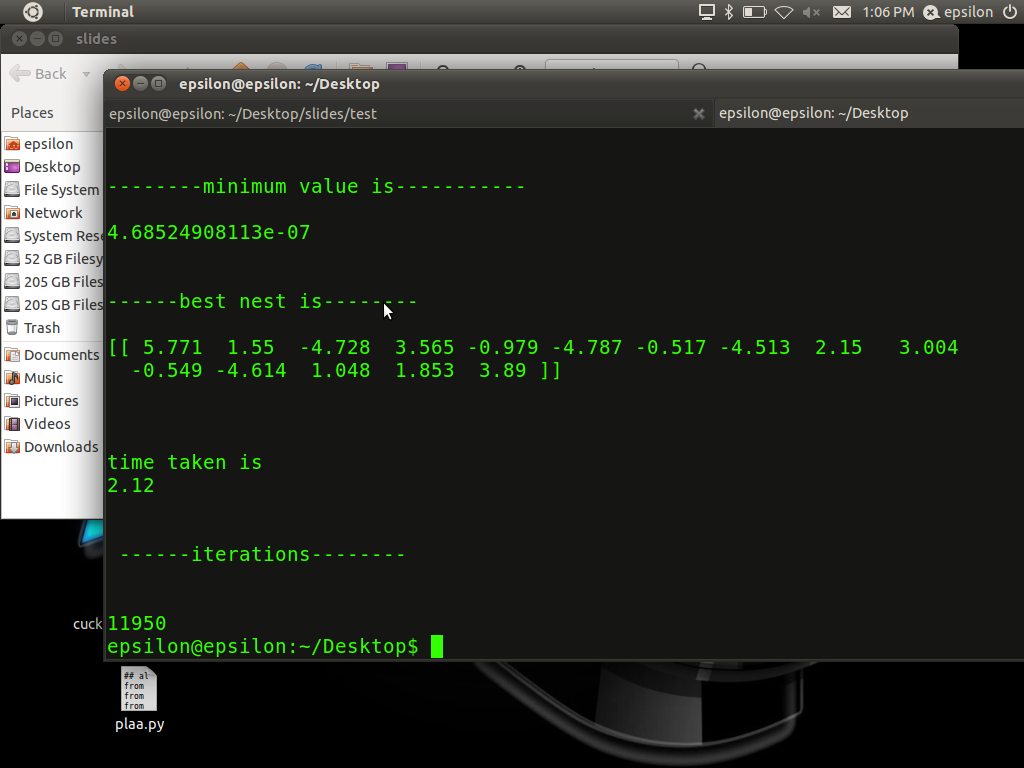
\includegraphics[width=0.85\textwidth]{abc.png}
	\end{center}
\end{frame}

\begin{frame}
	\frametitle{Screen Shots}
	\textbf{GUI Interface}
	\begin{center}
	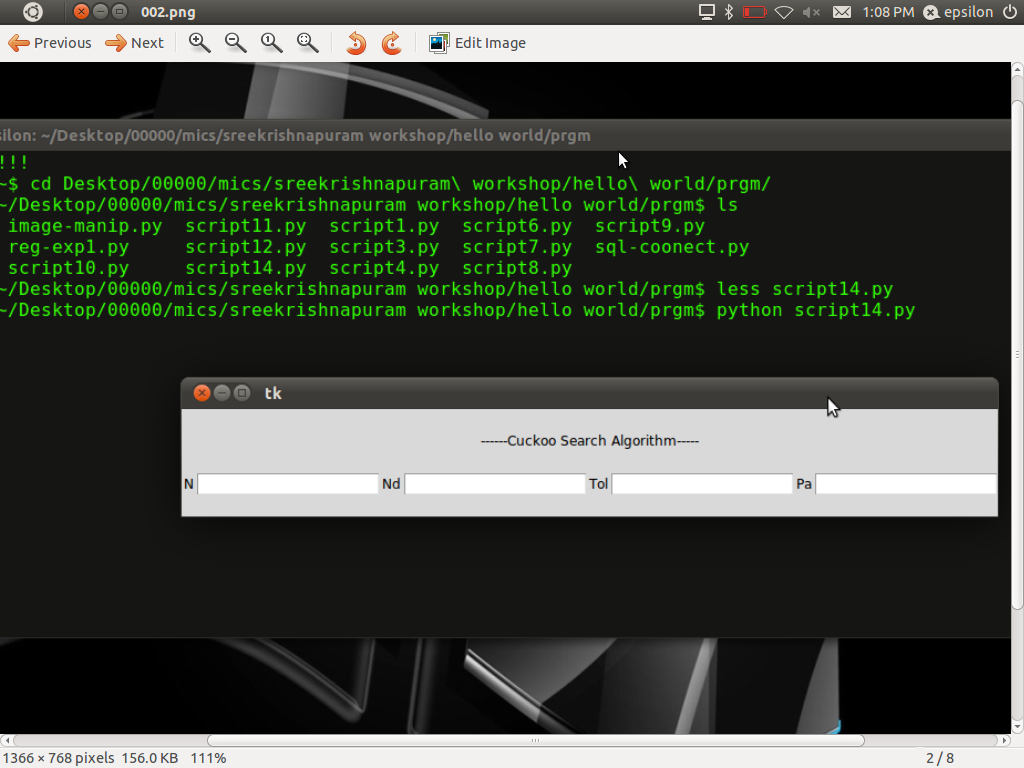
\includegraphics[width=0.85\textwidth]{abb.png}
	\end{center}
\end{frame}

%-21-%
\begin{frame}
  \begin{columns}
    \begin{column}{0.2\textwidth}
      Thank you!
    \end{column}
  \end{columns}
\end{frame}
\end{document}
